\subsection{Toy example - Synthetic Dataset}
\label{section:results-toy}
First experiments were run on synthetic data to validate the method. The workflow allows to build a dataset containing 1000 samples with custom number of relevant features (F), redundant features (R), copies (C) and noise (N). Rival features are created from items $\in$ F, an numbered in the same manner, e.g. A copy of F01 is named C01 and can be seen as a perfect rival feature. Redundant and rival features are our main aim, and are built as the square/cosinus of F features. The generated values are uniform random and the target is build using only items $\in$ F, so noise features are statistically independent from relevant ones.
% cuantas muestras? y variables

After swapping, the results are observed in Figure \ref{fig:triade}. Desired behaviours are listed below:

\begin{itemize}
    \item Features $\in$ F are not related to each other in the diagram, therefore discrimination performs well.
    \item Copied features behave as expected, since they hold a perfect (mutual) relation to their informative features. Again, copies are not related among them.
    \item Redundant features consistent in terms of relation, i.e. they are related to their Original feature’ copies, and other redundant. E.g. R02 to F02, C02 and Cos02.
    \item Noise (N) features do not establish any relation, which confirms their independence.
\end{itemize}

Figure \ref{fig:triade} presents three visualisations of the rivalry relations between variables.
% Triade
\begin{figure}[!hb]
	\centering
	\begin{subfigure}[b]{0.3\linewidth}
		\includegraphics[width=\linewidth]{figures/chords/chord_swap_Ensemble1000_RCN5333300_097.png}
		\caption{Chord diagram representation at \emph{t} = 0.98}
	\end{subfigure}
	\hfill
	\begin{subfigure}[b]{0.3\linewidth}
		\includegraphics[width=\linewidth]{figures/heatmaps/heatmap_swap_Ensemble1000_RCN5333300_097.png}
		\caption{Heatmap from matrix at \emph{t} = 0.98. Edge thickness indicates relation strength.}
	\end{subfigure}
	\hfill
	\begin{subfigure}[b]{0.3\linewidth}
		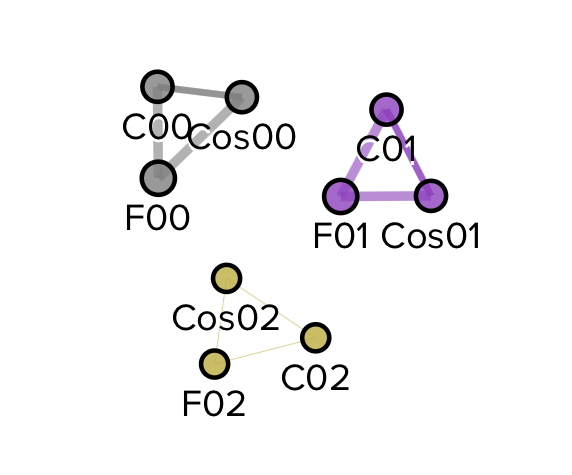
\includegraphics[width=\linewidth]{Minor Thesis/figures/graphs/graph-toy.png}
		\caption{Graph clustering at \emph{t} = 0.98}
	\end{subfigure}
	\caption{Clustering process. (a) Shows relation in Chord diagram to ease visualisation. (b) Gives the matrix which we post-process to keep only relevant links. (c) Final relation graph. Each connected component is a final group whose representative is the most connected node. Community detection algorithms colour each group.}
	\label{fig:triade}
\end{figure}

Overall, the new swapped predictions tend to have a lower accuracy (Suppl. Figure \ref{fig:gainloss}). Some redundant features relate to other than theirs. E.g R00 relates to F01, F02, although the relation is stronger to F00. This effect occurs due to randomness, since small sample sets, might arise similarities. We correct it using threshold filtering, allowing only relations above 0.97 get past it. Evolution of the relations using a moving threshold can be found in Suppl. Figure \ref{fig:six-chords}.
\\

Using a controlled dataset, we could validate the expected behaviour of the algorithm. Next, we present the analysis based on a real set of data.

\subsection{Type 2 Diabetes - Real Dataset}
Scripts applied to the Type 2 Diabetes (T2D) deliver results which can be interpreted using biological background. At a more in depth level, and taking into account the capabilities of the system, we pay attention not only to the results, but to the kind of data.
\\

A regular swapping run on an Ensemble containing T2D data takes 984$\times$3$\times$8$\times$298 = 7,037,568 swap attempts (Eq. in \ref{section:methods:complex}), being 984 the number of sequentials, 3 splits of data each, 8 original variables and 298 top variables to swap.
\\
% Rival variants graph
\begin{figure}[!ht]
    \centering
% 	\captionsetup{justification=centering}
	\begin{subfigure}[b]{0.30\linewidth}
		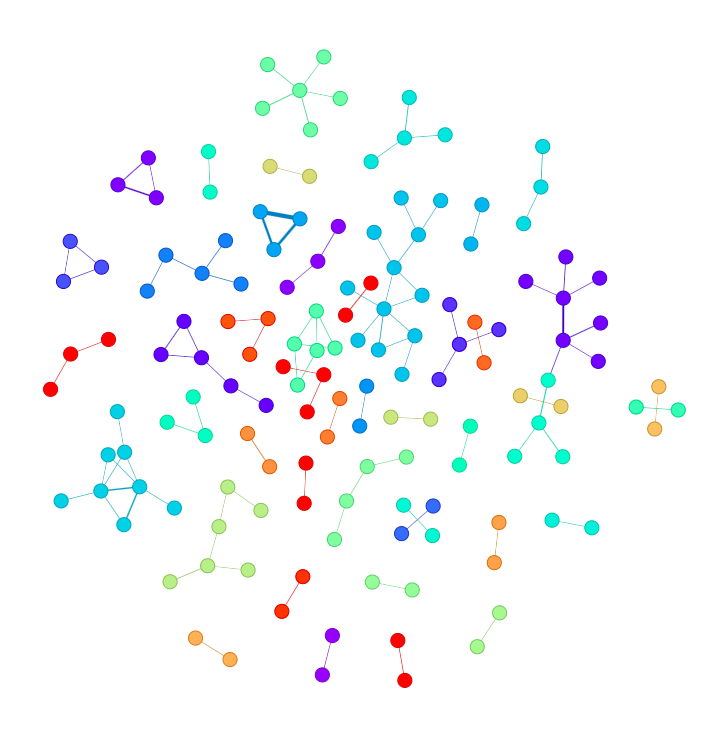
\includegraphics[width=\linewidth]{Minor Thesis/figures/graphs/main/g95102028.png}
		\caption{10\% cases min.}
	\end{subfigure}
	\hfill
	\begin{subfigure}[b]{0.30\linewidth}
		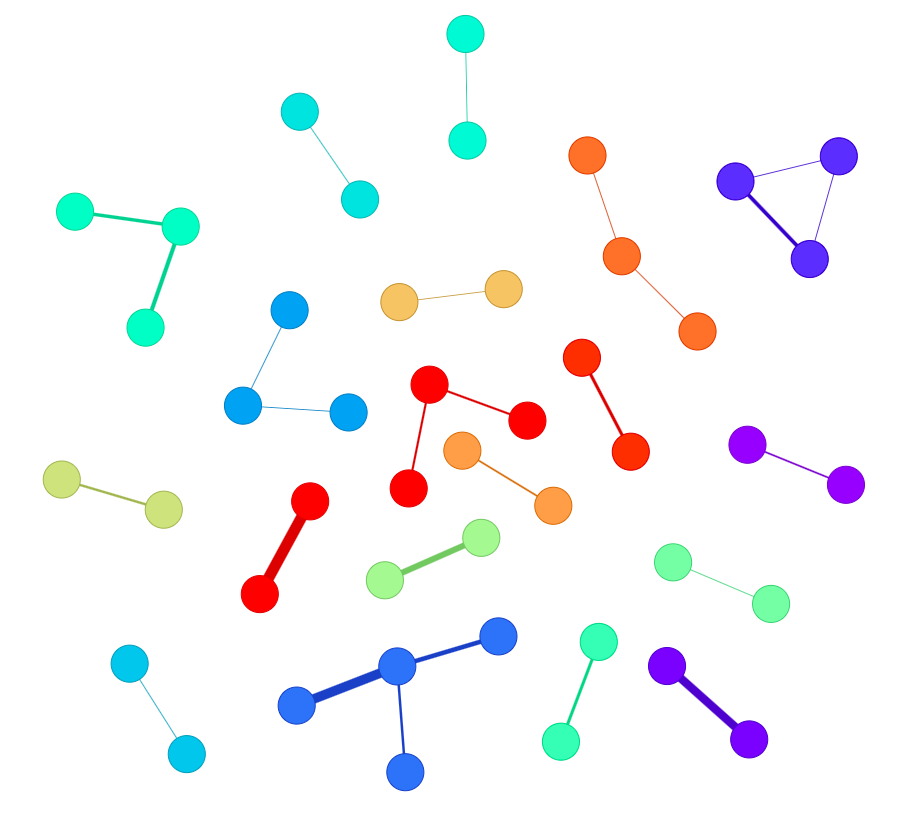
\includegraphics[width=\linewidth]{Minor Thesis/figures/graphs/main/g95202028.png}
		\caption{20\% cases min.}
	\end{subfigure}
	\hfill
	\begin{subfigure}[b]{0.30\linewidth}
		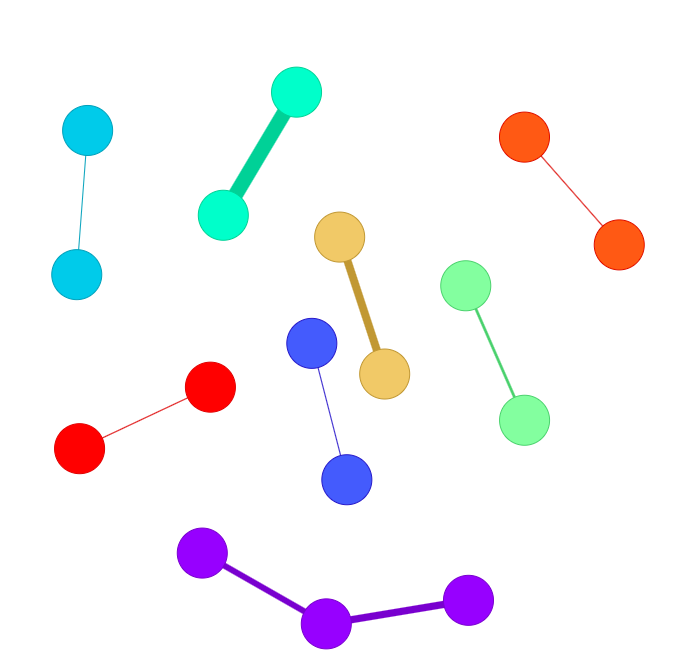
\includegraphics[width=\linewidth]{Minor Thesis/figures/graphs/main/g95302028.png}
		\caption{30\% cases min.}
	\end{subfigure}
	\hfill
    \caption{Rival variants graph. Each edge indicates the Rivalry Score among two variables. Colonies on Swap Score minimum = 0.95, 0.2 < Spearman Correlation < 0.8. (a) Discards variables whose original values are different less than 10\% of the feature's mode value, (b) does it on < 20\% and (c) on 30\%.}
    \label{fig:main-graphs}
\end{figure}

Normalised scores show the following pattern: when plotting the graph step by step -- filtering edge weight from the highest to the lowest-- , the variables added tend to have a $\approx$ 0.98 Spearman correlation similarity in the original data. Besides, for each addition, we add a node to the connected component and do not form new ones. If any Connected Component (CC) is created, it is soon linked. See Suppl. Figure \ref{fig:graph-evo-sa} for graph evolution.
\\

% Not-normalised scores show the same pattern, except the node additions is more exponential, i.e. it does not add one node at the time, but several.
% Testing the Correlation score among feature's values by randomly picking 10.000 samples, shows a bimodal distribution: either the Correlation is close to 0.9 or to 0.1, which might be causing the bias in the swapper. See Suppl. Figure \ref{fig:graph-evo-nn} for graph evolution.
% \\

% results table
\begin{table}[!hb]
\centering
\resizebox{\textwidth}{!}{%
\begin{tabular}{|c|c|c|c|c|c|c|}
\hline
\textbf{id}      & \textbf{reference\_count} & \textbf{grouped\_count} & \textbf{group}                         & \textbf{reference\_rank} & \textbf{grouped\_rank} & \textbf{pos\_changed} \\ \hline
SNP\_1           & 46                        & 50                      & \cellcolor[HTML]{47C1E5}756            & 19                       & 17                     & 2                     \\ \hline
\textbf{SNP\_2}  & \textbf{4}                & \textbf{50}             & \cellcolor[HTML]{47C1E5}\textbf{756}   & \textbf{55}              & \textbf{24}            & \textbf{31}           \\ \hline
SNP\_3           & 8                         & 9                       & \cellcolor[HTML]{63F6BF}2016           & 51                       & 62                     & -11                   \\ \hline
\textbf{SNP\_4}  & \textbf{1}                & \textbf{9}              & \cellcolor[HTML]{63F6BF}\textbf{2016}  & \textbf{58}              & \textbf{64}            & \textbf{-6}           \\ \hline
SNP\_5           & 30                        & 36                      & \cellcolor[HTML]{E73E25}2204           & 29                       & 28                     & 1                     \\ \hline
\textbf{SNP\_6}  & \textbf{6}                & \textbf{36}             & \cellcolor[HTML]{E73E25}\textbf{2204}  & \textbf{53}              & \textbf{34}            & \textbf{19}           \\ \hline
SNP\_7           & 21                        & 26                      & \cellcolor[HTML]{EDBF55}3508           & 38                       & 40                     & -2                    \\ \hline
\textbf{SNP\_8}  & \textbf{5}                & \textbf{26}             & \cellcolor[HTML]{EDBF55}\textbf{3508}  & \textbf{54}              & \textbf{46}            & \textbf{8}            \\ \hline
SNP\_9           & 40                        & 41                      & \cellcolor[HTML]{6FF58E}3907           & 22                       & 23                     & -1                    \\ \hline
\textbf{SNP\_10} & \textbf{1}                & \textbf{41}             & \cellcolor[HTML]{6FF58E}\textbf{3907}  & \textbf{58}              & \textbf{31}            & \textbf{27}           \\ \hline
SNP\_11          & 12                        & 21                      & \cellcolor[HTML]{343DFA}5884           & 47                       & 51                     & -4                    \\ \hline
SNP\_12          & 9                         & 21                      & \cellcolor[HTML]{343DFA}5884           & 50                       & 52                     & -2                    \\ \hline
SNP\_13          & 17                        & 25                      & \cellcolor[HTML]{8833FB}9115           & 42                       & 43                     & -1                    \\ \hline
\textbf{SNP\_14} & \textbf{6}                & \textbf{25}             & \cellcolor[HTML]{8833FB}\textbf{9115}  & \textbf{53}              & \textbf{47}            & \textbf{6}            \\ \hline
\textbf{SNP\_15} & \textbf{2}                & \textbf{25}             & \cellcolor[HTML]{8833FB}\textbf{9115}  & \textbf{57}              & \textbf{49}            & \textbf{8}            \\ \hline
SNP\_16          & 22                        & 29                      & \cellcolor[HTML]{E62E25}10209          & 37                       & 36                     & 1                     \\ \hline
\textbf{SNP\_17} & \textbf{7}                & \textbf{29}             & \cellcolor[HTML]{E62E25}\textbf{10209} & \textbf{52}              & \textbf{42}            & \textbf{10}           \\ \hline
\end{tabular}%
}
\caption{Re-ranked table including only features whose rank has changed. \emph{Reference count} column indicates the original votes obtained by the feature, while \emph{Grouped\_count} displays the new votes after grouping. The 8 different formed groups can also be seen in Figure \ref{fig:main-graphs} (c). Table's column \emph{group} colours match found groups. Bold rows mark features promoted to the existing top-ranked set. Parameters used: Swap Score=0.95, QLOI=0.3.}
\label{tbl:rerank}
\end{table}

Finally, on normalised scores corrected for quasi-constancy, a majority of CC containing 2 and 3 nodes is found. Figure \ref{fig:main-graphs} displays how the graph become less crowded as we increase the Rivalry Score and the QLOI thresholds.

% re-ranking
After generating the new relations file, i.e. establishing rivalry relations among variables, and hence grouping them when counting, we proceed to re-rank the list. The maximum value for the new votes assigned to a group is the sum of all the votes coming from the items belonging to this group, although due to the intersection subtraction (if present), it might be lower. Table \ref{tbl:rerank} shows an example of the re-ranking result.

\\

Analysing results extracted on this work configuration (Section \ref{section:cfg}), we observe the correlation among variables tends to be quite low (Suppl. Figure \ref{fig:triade-hist}), evidencing collisions among all-0's and all-1's column values. The Quasi-constant Leave-Out Index trims the node presence in the graph, however, it has no effect on correlation among variables. As a post-process step, we consider only the variables which hold a correlation close to 0.5, based on the fact that identical features containing quasi-constant values will have a correlation close to 1, and opposite features again containing quasi-constant values will have a correlation close to 0.
\\

Further analysis on Rivalry Scores of 0.975 and 1 can be found in Suppl. Material \ref{section:suppl:extra-hist}.
\\

Our main focus is put on rival variables which hold low similarity among them, but which in the context of a prediction, they become rival.

Based in an set of experiments, Table \ref{tbl:summary-exps} summarises changes occurring in the final list of relevant features after applying different configurations of the swapping algorithm.

% experiments table
\begin{table}[!hb]
\centering
\resizebox{\textwidth}{!}{%
\begin{tabular}{|c|c|c|c|c|}
\hline
\rowcolor[HTML]{EFEFEF} 
\textbf{Swap Score}  & \textbf{Quasi-constant leave-out index} & \textbf{Rank Changed} & \textbf{New in Top} & \textbf{New Top Total} \\ \hline
                        & 0.1                                     & 19                    & 4                   & 302                    \\ \cline{2-5}
                        & 0.2                                     & 2                     & 0                   & 298                    \\ \cline{2-5} 
\multirow{-3}{*}{1}     & 0.3                                     & -                     & -                   & 298                    \\ \hline
                        & 0.1                                     & 62                    & 23                  & 321                    \\ \cline{2-5}
                        & 0.2                                     & 15                    & 4                   & 302                    \\ \cline{2-5}
\multirow{-3}{*}{0.975} & 0.3                                     & -                     & -                   & 298                    \\ \hline
                        & 0.1                                     & 146                   & 77                  & 375                    \\ \cline{2-5} 
                        & 0.2                                     & 46                    & 22                  & 320                    \\ \cline{2-5} 
\multirow{-3}{*}{0.95}  & 0.3                                     & 18                    & 9                   & 307                    \\ \hline
\end{tabular}%
}
\caption{Rank changes on different parameters of swapper results. \emph{Quasi-constant index} (QLOI) indicates the percentage of values different from the feature's mode minimum required (0.1 = 10\%). \emph{Rank changed} depicts how many nodes have changed their rank in the list, according to the new relations. Some features have entered the old top298 group which hold more than 8 votes, therefore the result set increases and some features are re-ranked gaining relevance.}
\label{tbl:summary-exps}
\end{table}